\documentclass[a4paper,11pt]{article}

%% Language and font encodings
\usepackage[italian]{babel}
\usepackage[utf8]{inputenc}
\usepackage[T1]{fontenc}
\usepackage{caption}
\usepackage{subcaption}
\usepackage{float}

%% Sets page size and margins
\usepackage[a4paper,top=3cm,bottom=3cm,left=3cm,right=3cm]{geometry}

%% Useful packages
\usepackage{graphicx}
\usepackage{xcolor}
\usepackage{listings}
\usepackage{url}
\usepackage{chapterbib}

%% Define swift language
\lstdefinelanguage{swift}
{
  morekeywords={
  func,if,then,else,for,in,while,do,switch,case,default,where,break,continue,return,import,struct,class,enum,var,func,let,init,self,override,final,private,static
  },
  morecomment=[l]{//}, % l is for line comment
  morecomment=[s]{/*}{*/}, % s is for start and end delimiter
  morestring=[b]" % defines that strings are enclosed in double quotes
}

%% Renew commands
\renewcommand{\lstlistingname}{}
\renewcommand{\figurename}{Figura}

%% Hide subsections from the table of contents
\setcounter{tocdepth}{2}

\definecolor{keyword}{HTML}{BA2CA3}
\definecolor{string}{HTML}{D12F1B}
\definecolor{comment}{HTML}{008400}

% Python
\lstset{
  language=python,
  basicstyle=\ttfamily,
  showstringspaces=false, % lets spaces in strings appear as real spaces
  columns=fixed,
  keepspaces=true,
  keywordstyle=\color{keyword},
  stringstyle=\color{string},
  commentstyle=\color{comment},
}

% Swift
\lstset{
  language=swift,
  basicstyle=\ttfamily,
  showstringspaces=false, % lets spaces in strings appear as real spaces
  columns=fixed,
  keepspaces=true,
  keywordstyle=\color{keyword},
  stringstyle=\color{string},
  commentstyle=\color{comment},
}

%% Begin document

\begin{document}

\title{

\includegraphics[height=30mm]{./unifi/stemma}~\\[0.5cm]
\LARGE Confronto tra diversi tool di Named Entity Recognition su testo in linguaggio naturale \\[0.5cm]
\normalsize Elaborato di Security and Knowledge Management (6 CFU)
}
\date{}
\maketitle

\tableofcontents
\clearpage

% Introduzione
\section{Introduzione}
Lo scopo di questo elaborato è quello di valutare e confrontare diversi tool per l'estrazione di entità nominate in testi sia in inglese che in italiano. 

Nel capitolo \ref{sec:ner} viene introdotto il processo di \textbf{NER} (\textit{Named Entity Recognition}) e viene fornita una panoramica sui principali approcci al problema, e il capitolo \ref{sec:entityextractors} illustra brevemente ciascuno dei tool utilizzati.

Nei capitoli \ref{sec:dataset} e \ref{sec:experiments} vengono descritti rispettivamente i due dataset utilizzati per gli esperimenti (inglese e italiano), i passaggi di preprocessamento dei dati e gli esperimenti realizzati. Infine, il capitolo \ref{sec:results} mostra i risultati ottenuti.

% Named Entity Recognition
\section{Named Entity Recognition (NER)}
\label{sec:ner}

L'elaborazione del linguaggio naturale (o \textbf{NLP, Natural Language Processing}), è un ambito dell’intelligenza artificiale che si occupa dei problemi legati all’analisi e all’elaborazione dei linguaggi naturali. \cite{wiki:nlp}
 
Al contrario dei linguaggi formali, utilizzati nell’interazione tra uomo e macchina, i linguaggi naturali non sono definiti da regole precise che ne permettono un’interpretazione univoca, ma presentano delle caratteristiche di \textbf{ambiguità} (eccezioni, sinonimi, figure retoriche, forme idiomatiche dipendenti fortemente dal contesto ecc...) che rendono il processo di elaborazione difficile e complesso. 

La ricerca in ambito NLP è rivolta principalmente allo studio di meccanismi di risoluzione di queste ambiguità, e di come possano essere riprodotti tramite algoritmi eseguibili dalle macchine.

Alcuni dei campi di cui si occupa NLP sono: 
\begin{itemize}
	\item \textit{Automatic Summarization}: la produzione automatica di un riassunto dei contenuti principali a partire da un testo;
	\item \textit{Information Extraction}: l'estrazione di informazioni semantiche da dati non strutturati, come ad esempio documenti di testo;
	\item \textit{Optical Character Recognition}: la ricostruzione di un testo tramite il rilevamento dei caratteri che lo compongono, a partire da un’immagine;
	\item \textit{Sentiment Analysis}: la costruzione di sistemi per l'identificazione ed estrazione di opinioni a partire da un testo;
	\item \textit{Speech Recognition}: sistemi di riconoscimento vocale per la trascrizione automatica di testo a partire da un file audio.
\end{itemize}

Fa parte dell'\textit{Information Extraction} anche l'\textit{estrazione di entità con nome} (o \textbf{Named Entity Recognition, NER}), un processo che cerca di trovare e classificare ogni singolo elemento presente in un testo all’interno di categorie predefinite come, ad esempio, persone, organizzazioni, luoghi o eventi. Questo processo è suddiviso come due problemi distinti: l'individuazione delle entità in una frase e la loro classificazione in base alle categorie alle quali appartengono. \cite{wiki:ner}

\begin{figure}[H]
\centering
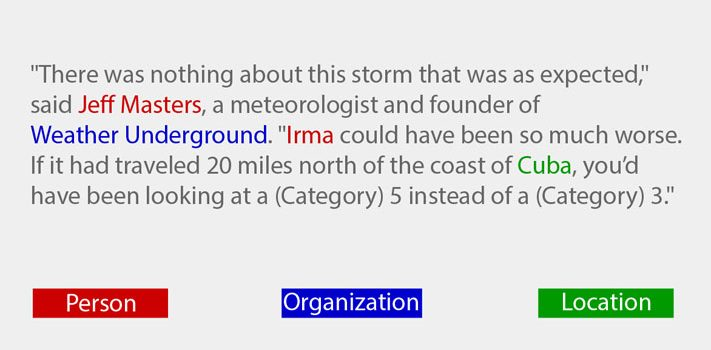
\includegraphics[width=0.6\textwidth]{img/ner}
\caption{Esempio di Named Entity Recognition in un testo in lingua inglese. (Fonte: \textit{opendatascience.com})}
\label{fig:results-it}
\end{figure}

I possibili approcci a entrambi i problemi possono essere di tre tipi:

\begin{itemize}
	\item Approccio basato su \textbf{lookup list}, quindi sul riconoscimento di parti del testo all’interno di liste predefinite suddivise per categorie. È un sistema semplice, ma che richiede liste estremamente complesse ed estese di possibili entità, difficili da mantenere; 
	\item Approccio basato su una \textbf{lista di regole} (\textit{rule-based}), in cui il testo viene analizzato secondo un insieme di regole grammaticali e sintattiche che determinano la presenza di entità all’interno di un testo. Come già illustrato in precedenza, la complessità e l'irregolarità del linguaggio umano rende molto difficile la stesura di regole che siano efficaci per qualsiasi contesto;
	\item Approccio \textbf{statistico}, attraverso l’uso di tecniche di \textbf{machine learning}. Questo approccio consiste nell’identificare \textit{pattern} specifici nei dati forniti in input per determinare in modo probabilistico dove potrebbe essere presente un’entità.
\end{itemize}

L'introduzione di tecniche di Machine Learning nel NLP, avvenuta intorno alla fine degli anni ‘80, e in particolare la possibilità di applicare modelli statistici all'analisi del linguaggio ha rappresentato una vera e propria rivoluzione nel settore. Un tipico approccio, basato su ML, consiste nel vedere NER come un problema di \textit{sequence tagging} per la categorizzazione, attraverso l’assegnamento di etichette degli elementi che compongono una data sequenza.
Alcuni esempi di modelli su cui si basano gli algoritmi utilizzati per questo tipo di task
sono \textit{Hidden Markov Models}, \textit{Maximum Entropy Markov Models}, \textit{Conditional Random Fields} e \textit{Support Vector Machines}. \cite{nlp-ner-tesi}
\newline
\newline
L'obiettivo di questo elaborato, quindi, è quello di provare e confrontare diversi tool per l'estrazione di entità, classificandoli in base alla performance e ai risultati ottenuti sullo stesso set di dati. Il capitolo \ref{sec:entityextractors} fornisce una panoramica su ciascuno dei tool utilizzati.

% Entity Extraction
\clearpage
\section{Estrattori di entità}
\label{sec:entityextractors}
Per questo elaborato sono stati individuati nove tool diversi per il riconoscimento di entità, elencati di seguito.

% Dandelion
\subsection{Dandelion}
\label{extractor:dandelion}
Dandelion (\textit{dandelion.eu}) è una piattaforma web che offre servizi di analisi semantica su testi in linguaggio naturale. \cite{dandelion}

Al momento lavora su testi in inglese, francese, tedesco, spagnolo, portoghese e italiano. Sono messe a disposizione diverse funzioni:

\begin{itemize}
	\item \textit{Estrazione di entità}: trova menzioni di luoghi, persone, marchi ed eventi in documenti e social media. Ottieni facilmente ulteriori dati sulle entità;
	\item \textit{Classificazione di testo e contenuto}: Classificare il testo multilingue in tassonomie standard predefinite o creare il proprio schema di classificazione personalizzato in pochi minuti;
	\item \textit{Analisi del sentimento}: Identificare se l'opinione espressa nei brevi testi (come le recensioni dei prodotti) è positiva, negativa o neutra;
	\item \textit{Similarità semantica}: confronta due testi e calcola la loro somiglianza sintattica e semantica, utile per capire ad esempio se riguardano lo stesso argomento.
\end{itemize}

In questo elaborato è stata utilizzata esclusivamente la funzione di estrazione di entità. Il servizio è gratuito per un uso limitato (fino a mille richieste al giorno), ed offre invece dei piani a pagamento per le aziende (a partire da 49\$ al mese).

Le API messe a disposizione richiedono un token di autenticazione, che viene indicato nella pagina del profilo dopo essersi registrati alla piattaforma web.

L'endpoint per le API è il seguente:
\newline

\textit{https://api.dandelion.eu/datatxt/nex/v1/}
\newline

E supporta i seguenti parametri:
\begin{itemize}
	\item \textit{text}: testo da analizzare (o, in alternativa, \textit{html} per passare direttamente codice html o \textit{url} per estrarre testo da un indirizzo web);
	\item \textit{token}: il token di autenticazione;
	\item \textit{lang}: lingua del testo da analizzare (de | en | es | fr | it | pt | ru | auto);
	\item \textit{top\_entities}: specifica il numero delle entità più importanti che devono essere incluse nella risposta. Se questo valore è maggiore di zero, verrà applicato un algoritmo di classificazione per ordinare tutte le entità in base alla loro importanza rispetto al testo di input e solo le più importanti verranno incluse nella risposta;
	\item \textit{min\_confidence}: specifica la soglia per il valore di confidenza: le entità con un valore di confidenza inferiore a questa soglia verranno eliminate. La fiducia è una stima numerica della qualità dell'annotazione, che varia tra 0 e 1. Una soglia più alta significa che si otterranno meno annotazioni ma più precise. Per questo elaborato è stato scelto di utilizzare un valore fissato a 0.75;
	\item \textit{social.hashtag}: serve per abilitare il supporto agli hashtag (\#), per analizzare correttamente tweet e post di \textit{Facebook};
	\item \textit{social.mention}: come per gli hashtag, ma abilita il supporto alle menzioni (@);
	\item \textit{include}: lista separata da virgola che indica quali ulteriori informazioni restituire sulle entità annotate: ad esempio "types" aggiunge informazioni sul tipo di entità da \textit{DBpedia}, "abstract" aggiunge il testo dell'estratto di \textit{Wikipedia}, "image" aggiunge un link a un'immagine dell'entità taggata, "lod" aggiunge collegamenti a entità equivalenti (sameAs) nei repository supportati di \textit{Linked Open Data}.\newline
\end{itemize}

\begin{lstlisting}[basicstyle=\small, language=python, frame=single, caption={Esempio di codice Python per l'estrazione di entità tramite le API di \textit{Dandelion}.},captionpos=b]
import requests

token = "XXX" # token di autenticazione
text = "Parigi e' la capitale della Francia." # testo da analizzare
base_url = 'https://api.dandelion.eu/datatxt/nex/v1/?lang=it \
            &min_confidence=0.75&token={}&text={}'.format(token, text)
json = requests.get(base_url).json()
list(set([entity['spot'] for entity in json['annotations']]))

# Output: ['Parigi', 'Francia']
\end{lstlisting}


% NL
\subsection{Natural Language framework}
\label{extractor:nl}
Natural Language è un framework nativo di Apple progettato che fornisce delle API per attività di elaborazione di linguaggio naturale su tutti i dispositivi proprietari. \cite{nl}

Il framework \textit{Natural Language} fornisce una varietà di funzionalità di elaborazione del linguaggio con supporto per tante lingue, tra cui inglese e italiano. Alcune di queste funzionalità sono:
\begin{itemize}
	\item \textit{Identificazione della lingua}, rilevamento automatico della lingua da un testo;
	\item \textit{Tokenizzazione}, suddivisione di un testo in unità linguistiche o token;
	\item \textit{Etichettatura delle parti del discorso}, marcatura di singole parole con la loro parte del discorso;
	\item \textit{Lemmatizzazione}, per ottenere la forma canonica di una parola in base alla sua analisi morfologica;
	\item \textit{Riconoscimento delle entità nominate}, identificando i token come nomi di persone, luoghi o organizzazioni;
	\item È inoltre possibile utilizzare questo framework per addestrare e distribuire modelli di linguaggio naturale personalizzati.\newline
\end{itemize}

Il framework richiede l'installazione del linguaggio di programmazione \textit{Swift}, compatibile al momento solo con sistemi \textit{macOS} e \textit{Linux}.

\clearpage
\begin{lstlisting}[basicstyle=\small, language=swift, frame=single, caption={Esempio di codice Swift per l'estrazione di entità tramite il framework \textit{Natural Language}.},captionpos=b]
import NaturalLanguage

// testo da analizzare
var text: String = "Parigi e' la capitale della Francia."

var entities: [String] = []
let tagger = NLTagger(tagSchemes: [.nameType])
tagger.string = text
tagger.enumerateTags(in: text.startIndex..<text.endIndex, 
		     unit: .word, scheme: .nameType, 
		     options: [.joinNames]) { (tag, range) -> Bool in
    switch tag {
        // entita': persone, luoghi o organizzazioni
        case .personalName?, .placeName?, .organizationName?:
            entities.append(String(text[range]))
        default: break
    }
    return true
}

// Output: entities = ['Parigi', 'Francia']
\end{lstlisting}

% Polyglot
\subsection{Polyglot}
\label{extractor:polyglot}
Polyglot è un altro tool open-source scritto in linguaggio \textit{Python} per l'elaborazione del linguaggio naturale con supporto ad un grande numero di lingue diverse, tra cui inglese e italiano. \cite{polyglot}

Supporta diverse funzionalità, tra cui:

\begin{itemize}
	\item Tokenizzazione (165 lingue);
	\item Rilevamento della lingua (196 lingue);
	\item Riconoscimento delle entità nominate (40 lingue);
	\item Etichettatura delle parti del discorso (16 lingue);
	\item Analisi del sentimento (136 lingue);
	\item Analisi morfologica (135 lingue);
	\item Traslitterazione (69 lingue).
\end{itemize}

Per il riconoscimento di entità, Polyglot riconosce 3 categorie di entità:

\begin{itemize}
	\item \textbf{Sedi} (Tag: \textit{I-LOC}): città, paesi, regioni, continenti, quartieri, divisioni amministrative...;
	\item \textbf{Organizzazioni} (Tag: \textit{I-ORG}): squadre sportive, giornali, banche, università, scuole, organizzazioni non profit, aziende...;
	\item \textbf{Persone} (Tag: \textit{I-PER}): politici, scienziati, artisti, atleti...\newline
\end{itemize}

\begin{lstlisting}[basicstyle=\small, language=python, frame=single, caption={Esempio di codice Python per l'estrazione di entità con \textit{Polyglot}.},captionpos=b]
from polyglot.text import Text

text = "Parigi e' la capitale della Francia." # testo da analizzare
blob = Text(text)
list(set([' '.join(entity) for entity in blob.entities]))

# Output: ['Parigi', 'Francia']
\end{lstlisting}

% Spacy
\subsection{Spacy}
\label{extractor:spacy}
spaCy è una libreria open source tra le più usate per l'elaborazione del linguaggio naturale, scritta in \textit{Python} e rilasciata sotto licenza \textit{MIT}. \cite{spacy} 

Attualmente \textit{Spacy} implementa modelli statistici di reti neurali in inglese, tedesco, spagnolo, portoghese, francese, italiano, olandese e greco; inoltre offre funzionalità di \textit{NER} e di tokenizzazione per diverse altre lingue. Supporta molte funzionalità, tra cui:

\begin{itemize}
	\item Tokenizzazione;
	\item Riconoscimento delle entità nominate;
	\item Supporto per oltre 59 lingue;
	\item 46 modelli statistici per 16 lingue;
	\item Etichettatura delle parti del discorso;
	\item Visualizzatori integrati per sintassi e \textit{NER};
	\item Facile integrazione con deep learning (supporto all''integrazione con \textit{TensorFlow}, \textit{PyTorch}, \textit{scikit-learn} e \textit{Gensim}).
\end{itemize}

I sui punti di forza sono la velocità, efficienza e la possibilità di costruire facilmente modelli statistici linguisticamente sofisticati per una varietà di problemi di \textit{NLP}.
\newline
\begin{lstlisting}[basicstyle=\small, language=python, frame=single, caption={Esempio di codice Python per l'estrazione di entità con \textit{Spacy}.},captionpos=b]
import spacy

text = "Parigi e' la capitale della Francia."  # testo da analizzare
nlp = spacy.load('it_core_news_sm')  # carica modello italiano
doc = nlp(text)
list(set([e.text for e in doc.ents]))

# Output: ['Parigi', 'Francia']
\end{lstlisting}

%NLTK
\subsection{Natural Language Toolkit (NLTK)}
\label{extractor:nltk}
NLTK (Natural Language Toolkit), è una suite di moduli \textit{Python} open source, dataset e tutorial che supportano la ricerca e lo sviluppo nell'elaborazione del linguaggio naturale. \cite{nltk}

\textit{NLTK} fornisce un'implementazione degli algoritmi più comuni in \textit{NLP} come la tokenizzazione, etichettatura di parti del discorso, stemming, analisi del sentimento, segmentazione e riconoscimento di entità nominate. È uno strumento molto potente che però non supporta la lingua italiana (almeno per il riconoscimento di entità).

\textit{NLTK} tra le altre cose punta anche supportare la ricerca e l'insegnamento dell'\textit{NLP} e di altri campi correlati, come la linguistica, le scienze cognitive, l'intelligenza artificiale, l'\textit{information retrieval}, e il \textit{machine learning}; è stato usato con successo come ausilio all'insegnamento, come strumento per lo studio individuale e come piattaforma per prototipare e sviluppare strumenti di ricerca. \cite{wiki:nltk}
\newline

\begin{lstlisting}[basicstyle=\small, language=python, frame=single, caption={Esempio di codice Python per l'estrazione di entità con \textit{NLTK}.},captionpos=b]
import nltk

# testo da analizzare
text = "Paris is the capital and largest city of France."

tokens = nltk.word_tokenize(text)
tagging = nltk.pos_tag(tokens)
named_entities = nltk.ne_chunk(tagging)
list(set([' '.join(w for w, t in elt) for elt in named_entities 
     if type(elt) == nltk.tree.Tree]))

# Output: ['Paris', 'France']
\end{lstlisting}

% Stanford
\subsection{Stanford CoreNLP}
\label{extractor:stanford-corenlp}
Stanford CoreNLP è un'implementazione Java di un \textit{Named Entity Recognizer}, che può essere invocata in \textit{Python} tramite la libreria \textit{NLTK} (vedi \ref{extractor:nltk}). È stato creato nel 2014 da \textit{Stanford NLP Group}, un team di docenti, programmatori e studenti dell'Università di Stanford che lavorano insieme su algoritmi che consentono ai computer di elaborare e comprendere i linguaggi umani.

\textit{Stanford CoreNLP} fornisce una serie di strumenti di analisi del linguaggio naturale. Dato in input un testo in linguaggio naturale, supporta la lemmatizzazione, l'etichettatura delle parti del discorso, il riconoscimento di entità e molto altro. È stato originariamente sviluppato per l'inglese, ma ora fornisce anche diversi livelli di supporto per arabo, cinese, francese, tedesco e spagnolo. Non supporta (per adesso) la lingua italiana.

Il codice di \textit{Stanford CoreNLP} è scritto in \textit{Java} ed è concesso in licenza con \textit{GNU General Public License v3}. \cite{stanford}
\newline

\begin{lstlisting}[basicstyle=\small, language=python, frame=single, caption={Esempio di codice Python per l'estrazione di entità con \textit{Stanford CoreNLP}.},captionpos=b]
import nltk
from nltk.tag import StanfordNERTagger

# testo da analizzare
text = "Paris is the capital and largest city of France."

# path del modello inglese e del jar di Stanford CoreNLP
model = './stanford/classifiers/english.muc.7class.distsim.crf.ser.gz'
jar = './stanford/stanford-ner.jar'

# Utilizza Stanford CoreNLP come tagger
tagger = StanfordNERTagger(model, jar)
tokens = nltk.word_tokenize(self.text)

chunk = []
entities = []
for token, tag in self.tagger.tag(tokens):
    if tag == 'O':
        # Concatena entita' parziali adiacenti, se necessario
        if chunk:
            entities.append(' '.join([c[0] for c in chunk]))
            chunk = []
    else:
        chunk.append((token, tag))

list(set(entities))

# Output: ['Paris', 'France']
\end{lstlisting}

% Stanza
\subsection{Stanza}
\label{extractor:stanza}
Stanza è un \textit{toolkit} di analisi del linguaggio naturale \textit{Python}, introdotto nel 2020 da \textit{Stanford NLP Group}, lo stesso team dietro alla libreria Java \textit{Stanford CoreNLP} (vedi \ref{extractor:stanford-corenlp}). \cite{stanza}

Rispetto ai toolkit ampiamente utilizzati, \textit{Stanza} presenta una pipeline completamente neurale indipendente dalla lingua per l'analisi del testo, e offre molte funzioni tra cui tokenizzazione, lemmatizzazione, etichettatura di parti del discorso e caratteristiche morfologiche, analisi delle dipendenze e riconoscimento di entità nominate. 

\textit{Stanza} è addestrato su un totale di 112 dataset di dati, e per il riconoscimento di entità supporta otto lingue: arabo, cinese, olandese, inglese, francese, tedesco, russo e spagnolo. Non supporta quindi per adesso la lingua italiana.
\newline

\begin{lstlisting}[basicstyle=\small, language=python, frame=single, caption={Esempio di codice Python per l'estrazione di entità con \textit{Stanza}.},captionpos=b]
import stanza

# testo da analizzare
text = "Paris is the capital and largest city of France."

nlp = stanza.Pipeline('en')  # carica modello inglese per l'analisi
doc = nlp(self.text)
list(set([e.text for e in doc.ents]))

# Output:  ['Paris', 'France']
\end{lstlisting}

% Tint
\subsection{Tint}
\label{extractor:tint}
Tint (\textit{The Italian NLP Tool}) è una pipeline open source basata su Java per l'elaborazione del linguaggio naturale esclusivamente in lingua italiana. \cite{tint}

Tint è basato su Stanford CoreNLP (vedi \ref{extractor:stanford-corenlp}) e può essere utilizzato come strumento autonomo, incluso come libreria Java o come servizio API REST. È anche distribuito su Maven Central, quindi può essere facilmente integrato in un progetto esistente.

Il \textit{NER} incluso in \textit{Tint} si basa sullo stesso classificatore incluso in \textit{Stanford CoreNLP} ed allenato sulla \textbf{Content Annotation Bank (I-CAB)} italiana, contenente circa 180.000 parole tratte dal quotidiano italiano \textit{L'Adige}, e utilizzato per il compito di \textit{Entity Recognition} di \textit{Evalita 2009}. \cite{dataset-it}

\textit{Tint} implementa la maggior parte degli strumenti linguistici comuni, come la codifica delle parti del discorso, l'analisi delle dipendenze, la tokenizzazione e il riconoscimento di entità. In questo elaborato, Tint è stato utilizzato come servizio \textit{API REST} (nel download è incluso uno script bash, \textit{tint-server.sh}, per l'avvio del server locale) che è in grado di restituire i risultati dell'analisi in formato \textit{JSON}.
\newline

\begin{lstlisting}[basicstyle=\small, language=python, frame=single, caption={Esempio di codice Python per l'estrazione di entità con \textit{Tint}.},captionpos=b]
import requests

# testo da analizzare
text = "Parigi e' la capitale della Francia."

# Il server Tint deve essere in esecuzione in locale nella porta 8012
base_url = 'http://localhost:8012/tint?text={}'.format(text)
json = requests.get(base_url).json()

entities = []
chunk = []
for sentence in json['sentences']:
    for token in sentence['tokens']:
        # entita': persone, luoghi o organizzazioni
        if token['ner'] in ['LOC', 'ORG', 'PER']:
            chunk.append(token)
        else:
            # Concatena entita' parziali adiacenti, se necessario
            if chunk:
                entities.append(' '.join([c['word'] for c in chunk]))
                chunk = []

# Output: entities = ['Parigi', 'Francia']
\end{lstlisting}

% Google Cloud
\subsection{Google Cloud}
\label{extractor:gcloud}
È possibile analizzare ed estrarre informazioni significative da testo non strutturato con le API di \textit{Natural Language} messe a disposizione dalla piattaforma \textit{Google Cloud}. \cite{gcloud}

\textit{Natural Language} utilizza la tecnologia di machine learning tramite modelli pre-addestrati per fornire funzionalità come analisi del sentimento, analisi ed estrazione delle entità, classificazione di contenuti e analisi della sintassi.

Al momento per l'estrazione di entità sono supportate dieci lingue: cinese (semplificato e tradizionale), inglese, francese, tedesco, italiano, giapponese, coreano, portoghese, russo e spagnolo.
\newline

L'utilizzo dell'API \textit{Natural Language} è a pagamento (pur offrendo 300\$ di credito ai nuovi iscritti), e il prezzo è calcolato mensilmente in base al numero di richieste effettuate. È richiesto un file \textit{json} di autenticazione che può essere scaricato direttamente dall'interfaccia web.

\clearpage
\begin{lstlisting}[basicstyle=\small, language=python, frame=single, caption={Esempio di codice Python per l'estrazione di entità con \textit{Google Cloud}.},captionpos=b]
from google.cloud import language_v1
from google.cloud.language_v1 import enums

# testo da analizzare
text = "Parigi e' la capitale della Francia."

# Autenticazione
client = language_v1.LanguageServiceClient
                    .from_service_account_file('auth.json')
                    
document = { "content": text, "type": enums.Document.Type.PLAIN_TEXT }
response = client.analyze_entities(document, enums.EncodingType.UTF8)

list(set([entity.mentions[0].text.content for e in response.entities
          if enums.Entity.Type(e.type).name in 
                  # entita': persone, luoghi o organizzazioni
                  ['PERSON', 'LOCATION', 'ORGANIZATION']
          and enums.EntityMention.Type(e.mentions[0].type).name 
                   == 'PROPER'
        ])
    )
)

# Output: ['Parigi', 'Francia']
\end{lstlisting}

% Dataset
\section{Dataset scelti}
\label{sec:dataset}
Sono stati scelti due dataset già annotati con entità, uno in lingua inglese e uno in lingua italiana, descritti di seguito.

% Dataset ENG
\subsection{Dataset in lingua inglese}
\label{ssec:dataset_en}
Il dataset inglese è stato scaricato da \textit{Kaggle}, una comunità online di data scientist e professionisti dell'apprendimento automatico che consente, tra le altre cose, di condividere ed esplorare set di dati. \cite{dataset-en}

Si tratta di un estratto del corpus \textbf{Groningen Meaning Bank} (\textit{GMB}), una risorsa semantica composta da oltre 10.000 testi in lingua inglese, tutti di pubblico dominio e disponibili gratuitamente per scopi di ricerca, già annotati appositamente per addestrare dei classificatori per la previsione di entità nominate.

Il file ha estensione \textit{.csv} e pesa circa 15MB, ed è strutturato in questo modo:
\begin{itemize}
	\item Il documento è suddiviso in frasi, identificate dalla colonna "\textit{Sentence \#}". Sono presenti oltre 45.000 frasi;
	\item Ogni riga rappresenta una parola della frase (ad esempio, la prima frase occupa 23 righe);
	\item La colonna \textit{Word} contiene la parola della frase;
	\item La colonna \textit{POS} indica la \textit{Part of Speech} della parola, ovvero la classe morfologica (sostantivo, verbo, aggettivo, ecc..) a cui appartiene;
	\item La colonna \textit{Tag} indica il \textit{tag} associato alla parola, ovvero il tipo di entità che rappresenta: in questo caso siamo interessati ai tag \textit{B-geo} (luogo), \textit{B-per} (persona) e \textit{B-org} (organizzazione). Se la parola non corrisponde a nessun tipo di entità viene indicato "\textit{O}" come tag.
\end{itemize}

\begin{figure}[H]
\centering
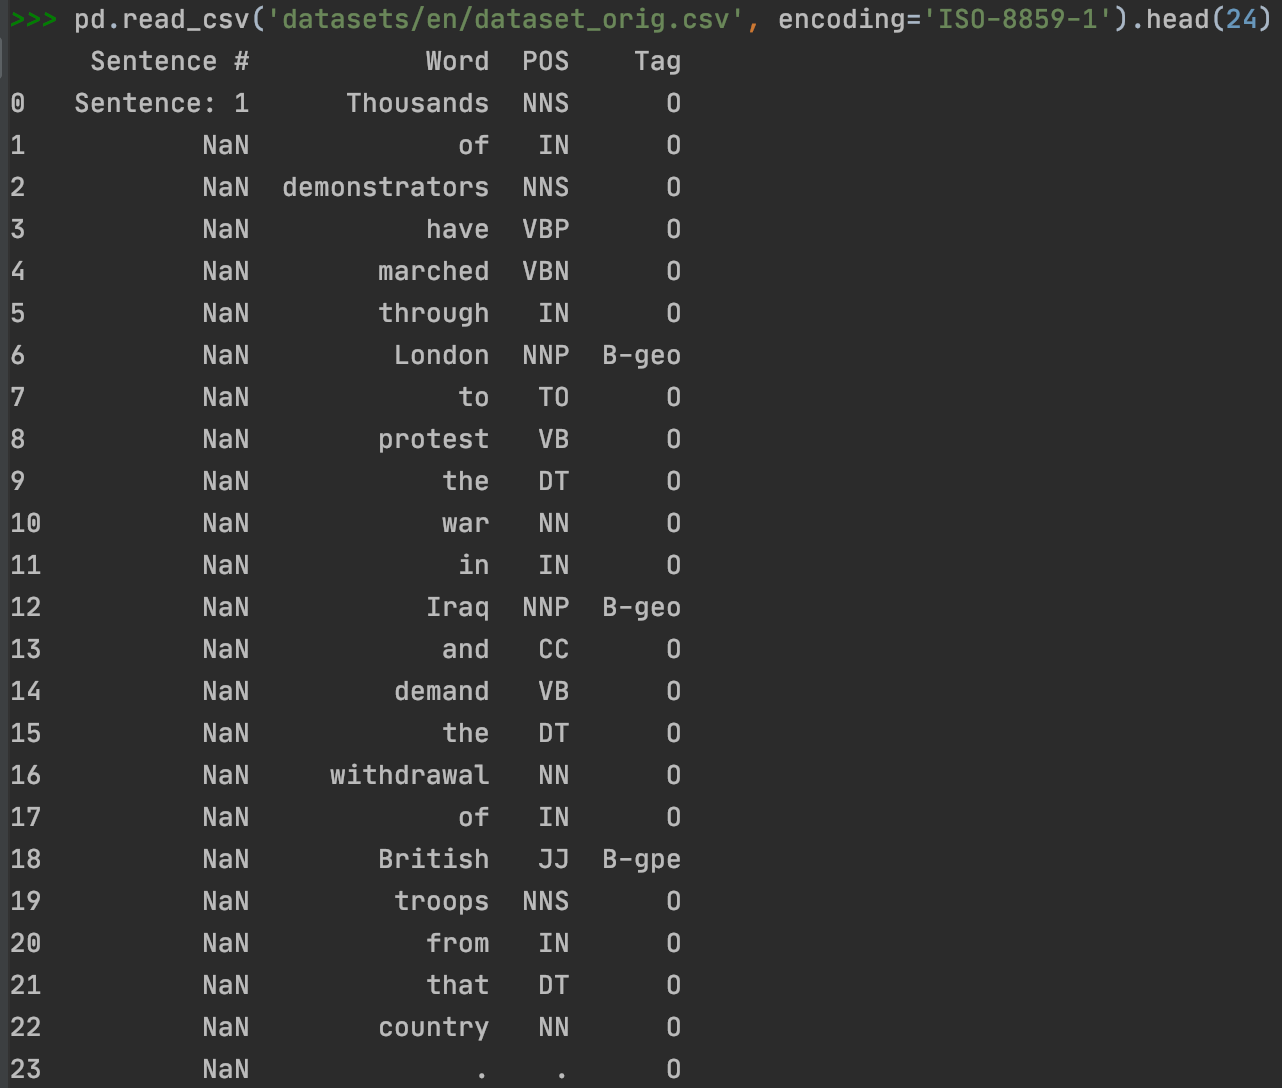
\includegraphics[width=0.7\textwidth]{img/dataset-en-orig}
\caption{Dataset inglese originale.}
\label{fig:dataset_en_orig}
\end{figure}

Le entità nominate sono annotate nel formato \textbf{IOB2}: il tag "B" (da "begin") indica il primo token dell'entità, mentre il tag "I" (da "inside") viene utilizzato per tutti gli altri token della stessa entità, se presenti (ad esempio, se l'entità è "\textit{Barack Obama}", la parola "\textit{Barack}" avrà token \textit{B-per} e "\textit{Obama}" avrà  \textit{I-per}). 
\newline

La figura \ref{fig:dataset_en_orig} mostra le prime 23 righe del dataset (corrispondenti alla prima frase del testo annotato - "\textit{Thousands of demonstrators have marched through London to protest the war in Iraq and demand the withdrawal of British troops from that country}."), e la colonna \textit{Tag}  evidenzia correttamente la presenza di tre entità geografiche (\textit{London}, \textit{Iraq}, \textit{British}).

\subsubsection{Preprocessamento dei dati}
Può risultare scomodo caricare tutte le volte in memoria un dataset con centinaia di migliaia di righe: si è resa quindi necessaria una fase intermedia di preprocessamento dei dati:

\begin{itemize}
	\item Sono state prese in considerazione solo le prime 25.000 righe del dataset originale;
	\item è stato scelto di associare una riga ad ogni frase del testo in modo da ridurre significativamente il numero di righe;
	\item La entità sono state raggruppate in un elenco unico per ciascuna frase;
	\item Sono state rimosse direttamente le frasi senza entità (inutili ai fini dell'elaborato).
\end{itemize}

Il risultato finale è esportato in un file \textit{.csv} di soli 130kb contenente poco più di 1100 righe, e strutturato come mostrato in figura \ref{fig:dataset_en_cleaned}.
\newline
\begin{figure}[H]
\centering
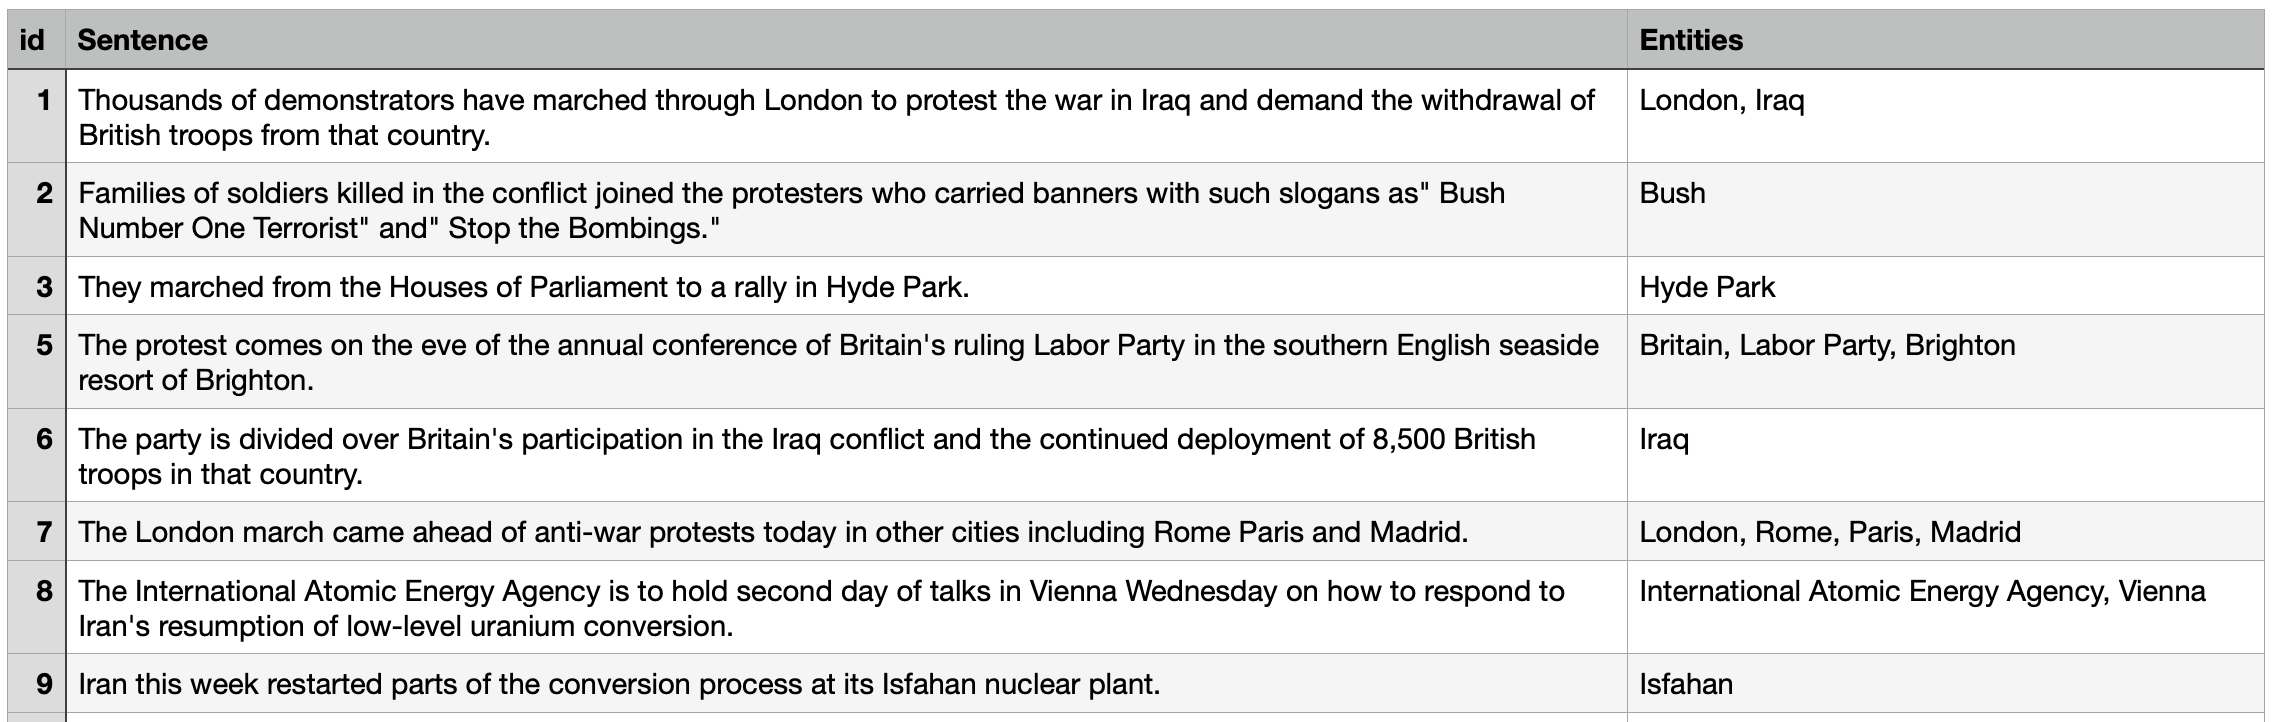
\includegraphics[width=1\textwidth]{img/dataset-en-cleaned}
\caption{Dataset inglese finale.}
\label{fig:dataset_en_cleaned}
\end{figure}

% Dataset ITA
\subsection{Dataset in lingua italiana}
Il dataset italiano è un estratto dell'\textbf{Italian Content Annotation Bank} (\textit{I-CAB}), un corpus annotato composto da 525 notizie tratte dal quotidiano locale \textit{L'Adige}, per un totale di circa 180.000 parole. La risorsa è liberamente disponibile per scopi di ricerca, previa accettazione di un contratto di licenza (e una attesa di due settimane), pertanto il modello risultante non può essere utilizzato per scopi commerciali.
Il corpus è stato utilizzato, tra le altre cose, presso \textit{EVALITA 2007} e \textit{2009}, una campagna di valutazione periodica dello stato di avanzamento del \textit{Natural Language Processing} (\textit{NLP}) per la lingua italiana. \cite{dataset-it}
\newline

Il file ha estensione \textit{.iob2} e pesa 7,2 MB. È organizzato in questo modo:

\begin{itemize}
	\item Il documento è suddiviso in oltre 500 brevi articoli;
	\item Ogni riga rappresenta una parola della frase;
	\item La prima colonna contiene la parola della frase;
	\item La seconda colonna indica la \textit{Part of Speech} della parola, ovvero la classe morfologica (sostantivo, verbo, aggettivo, ecc..) a cui appartiene;
	\item La terza colonna indica l'\textit{id} della notizia de \textit{l'Adige} a cui appartiene l'articolo;
	\item La quarta colonna, infine, indica il \textit{tag} associato alla parola, ovvero il tipo di entità che rappresenta: in questo caso siamo interessati ai tag \textit{B-LOC} (luogo), \textit{B-PER} (persona) e \textit{B-ORG} (organizzazione). Se la parola non corrisponde a nessun tipo di entità viene indicato "\textit{O}" come tag.
\end{itemize}

\begin{figure}[H]
\centering
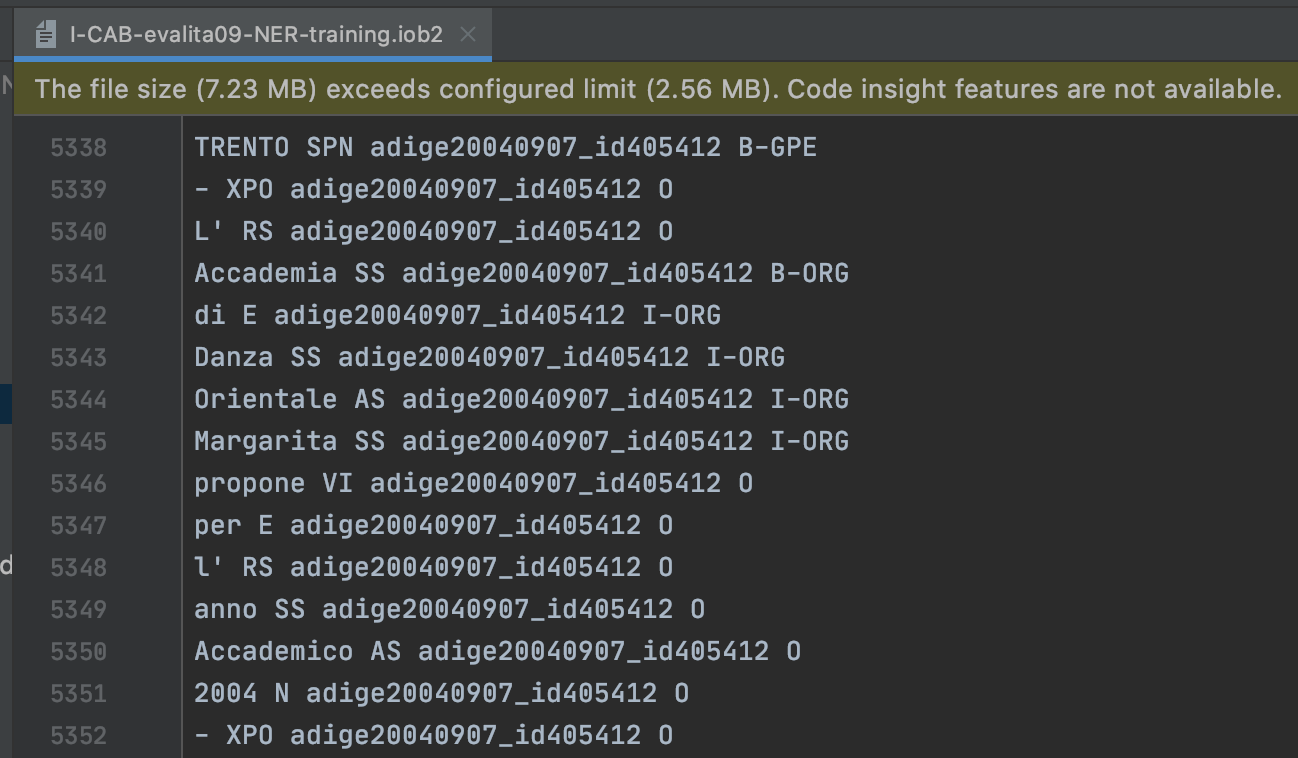
\includegraphics[width=0.7\textwidth]{img/dataset-it-orig}
\caption{Dataset italiano originale.}
\label{fig:dataset_it_orig}
\end{figure}

Anche per questo dataset le entità nominate sono annotate nel formato \textbf{IOB2} (vedi \ref{ssec:dataset_en}). La figura \ref{fig:dataset_it_orig} mostra un esempio di articolo annotato ("\textit{TRENTO - L'Accademia di Danza Orientale Margarita propone per l'anno Accademico 2004}") in cui sono individuate due entità (\textit{TRENTO} e \textit{Accademia di Danza Orientale Margarita}).

\subsubsection{Preprocessamento dei dati}
Anche in questo caso è stata applicata una fase intermedia di preprocessamento dei dati:

\begin{itemize}
	\item è stato scelto di associare una riga ad ogni frase dell'articolo, in modo da ridurre significativamente il numero di righe;
	\item La entità sono state raggruppate in un elenco unico per ciascuna frase;
	\item Sono state rimosse direttamente gli articoli senza entità e gli articoli con meno di dieci parole.
\end{itemize}

Il risultato finale è esportato in un file \textit{.csv} di circa 800kb contenente poco più di 10000 righe, e strutturato come mostrato in figura \ref{fig:dataset_it_cleaned}.

\begin{figure}[H]
\centering
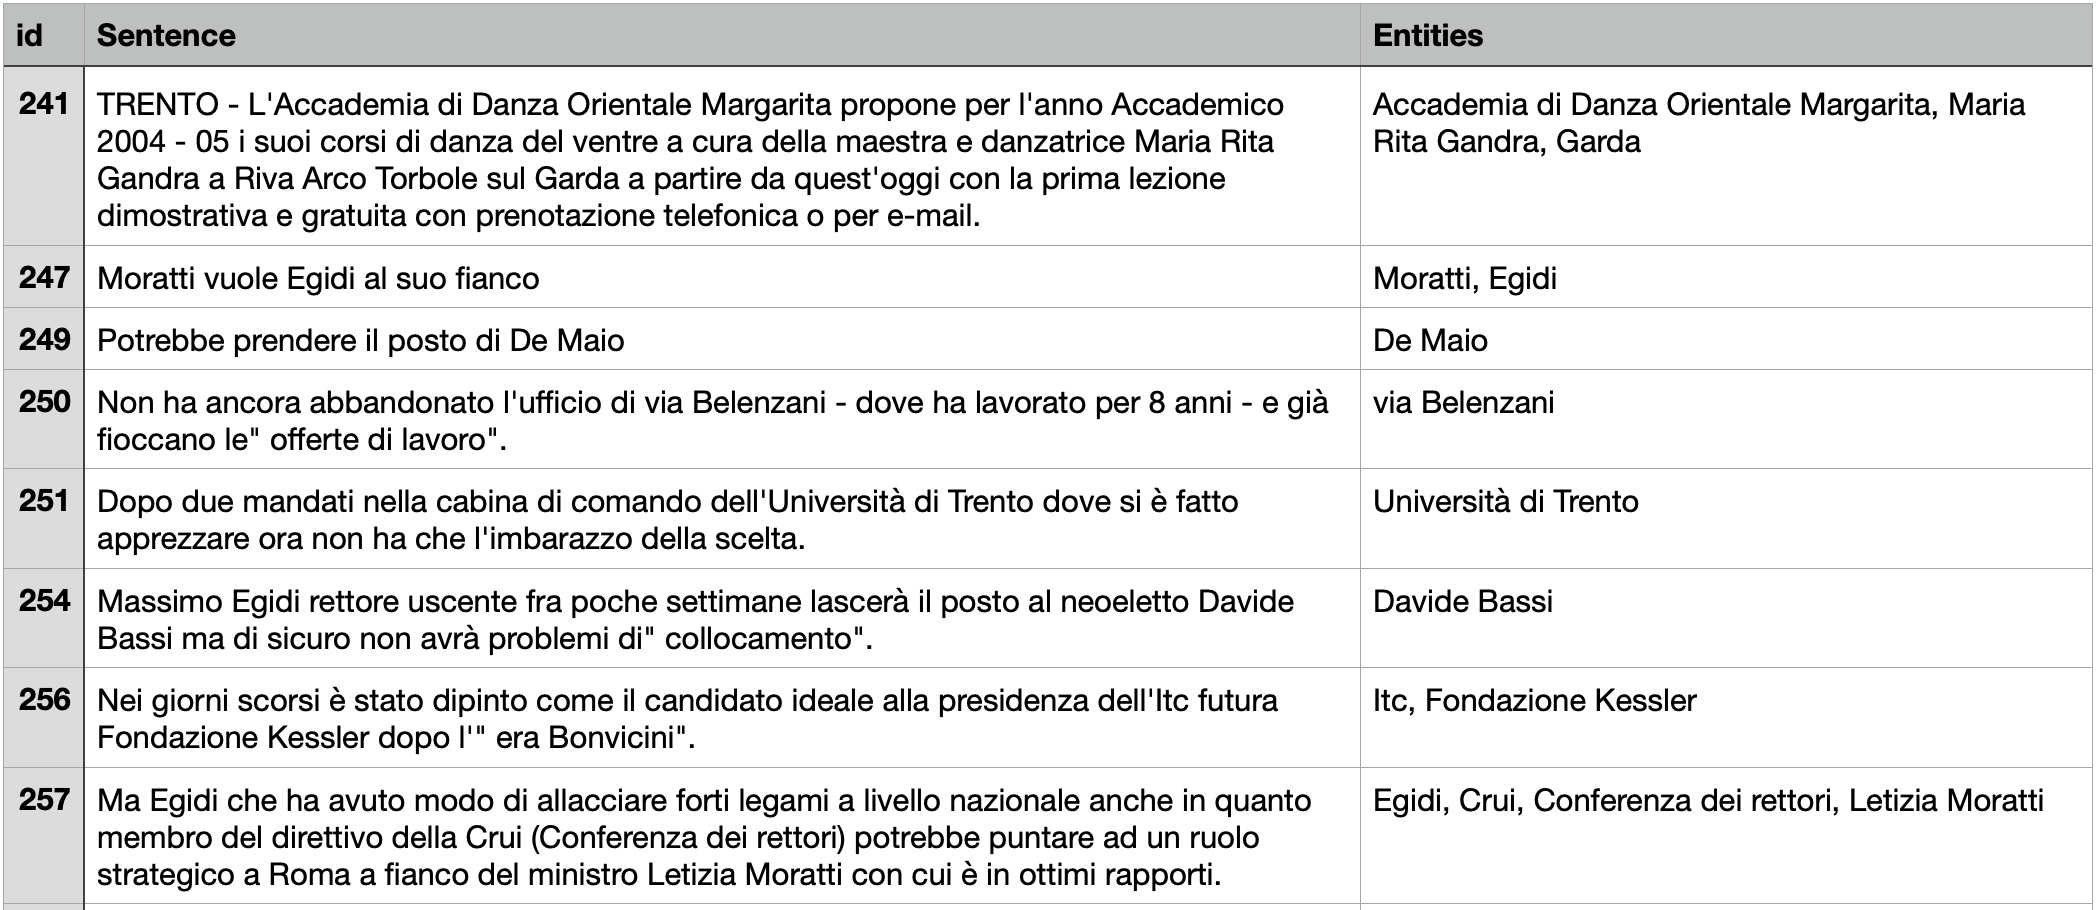
\includegraphics[width=0.9\textwidth]{img/dataset-it-cleaned}
\caption{Dataset italiano finale.}
\label{fig:dataset_it_cleaned}
\end{figure}

% Esperimenti
\addtocontents{toc}{\protect\setcounter{tocdepth}{1}}
\section{Esperimenti realizzati}
\label{sec:experiments}
Per una maggiore accuratezza gli esperimenti sono stati effettuati su 50 articoli in italiano e 50 in inglese. Ogni articolo è stato composto concatenando 10 frasi indipendenti tra loro.
Ciascun articolo è stato quindi salvato in un file \textit{.txt} all'interno della cartella del progetto (vedi figura \ref{fig:article_4}).

\begin{figure}[H]
\centering
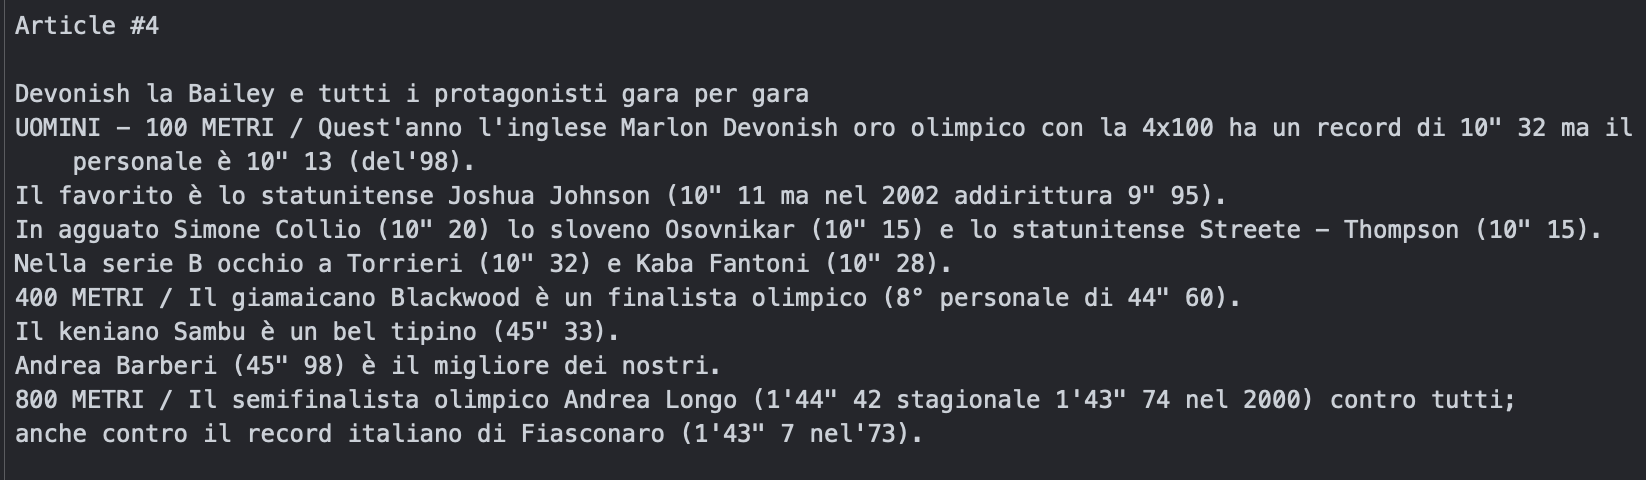
\includegraphics[width=1\textwidth]{img/article_4}
\caption{Esempio di articolo generato dal dataset italiano.}
\label{fig:article_4}
\end{figure}

\subsection{Valutazione della performance}
Il primo esperimento realizzato ha lo scopo di valutare la performance di ciascun estrattore di entità.
In lingua inglese sono stati valutati i seguenti tool: \textit{Spacy} (\ref{extractor:spacy}),  \textit{Polyglot} (\ref{extractor:polyglot}), \textit{Natural Language} (\ref{extractor:nl}), \textit{Dandelion} (\ref{extractor:dandelion}), \textit{NLTK} (\ref{extractor:nltk}), \textit{Stanford CoreNLP} (\ref{extractor:stanford-corenlp}), \textit{Google Cloud} (\ref{extractor:gcloud}) e \textit{Stanza} (\ref{extractor:stanza}).

Per l'italiano, invece, sono stati valutati ovviamente solo i tool che supportano la lingua: \textit{Spacy} (\ref{extractor:spacy}), \textit{Polyglot} (\ref{extractor:polyglot}), \textit{Natural Language} (\ref{extractor:nl}), \textit{Dandelion} (\ref{extractor:dandelion}), \textit{Tint} (\ref{extractor:tint}) e \textit{Google Cloud} (\ref{extractor:gcloud}).
\newline

Per ciascun articolo (50 in inglese e 50 in italiano), sono state estratte le entità con ogni tool.
A questo punto, conoscendo le entità "vere" per ogni articolo, è possibile definire i seguenti valori:

\begin{itemize}
  \item Falsi negativi (FN): numero di entità vere non estratte;
  \item Falsi positivi (FP): numero di entità estratte che però non corrispondono a nessuna tra quelle "vere";
  \item Veri negativi (TN): sarebbe il numero di entità "false" non estratte, ma è sempre zero nel nostro caso;
  \item Veri positivi (TP): numero di entità vere estratte correttamente.
\end{itemize}

\begin{figure}[H]
\centering
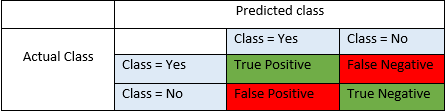
\includegraphics[width=0.9\textwidth]{img/table}
\caption{Esempio di matrice di confusione. (Fonte: \textit{blog.exsilio.com})}
\label{fig:table}
\end{figure}

\clearpage
Da cui è possibile definire le seguenti metriche:

\begin{itemize}
  \item \textbf{Accuracy}: è il rapporto tra il numero di entità corrette e il totale delle entità trovate ($\frac{TP+TN}{TP+FP+FN+TN}$);
  \item \textbf{Precision}: è il rapporto tra il numero di entità corrette e il totale delle entità estratte, includendo anche i falsi positivi ($\frac{TP}{TP+FP}$);
  \item \textbf{Recall}: è il rapporto tra il numero di entità corrette estratte e il totale delle entità presenti nell'insieme delle entità "vere" ($\frac{TP}{TP+FN}$);
  \item \textbf{F1 Score}: è la media armonica di
precision e recall ($2\cdot\frac{Recall \cdot Precision}{Recall + Precision}$).
\end{itemize}

I risultati trovati per ciascun articolo (tabella di comparazione delle entità, metriche e matrici di confusione) sono stati salvati nella cartella del progetto (vedi figura \ref{fig:entities_table}, \ref{fig:confusion_matrixes} e \ref{fig:results_ex}).

\begin{figure}[H]
\centering
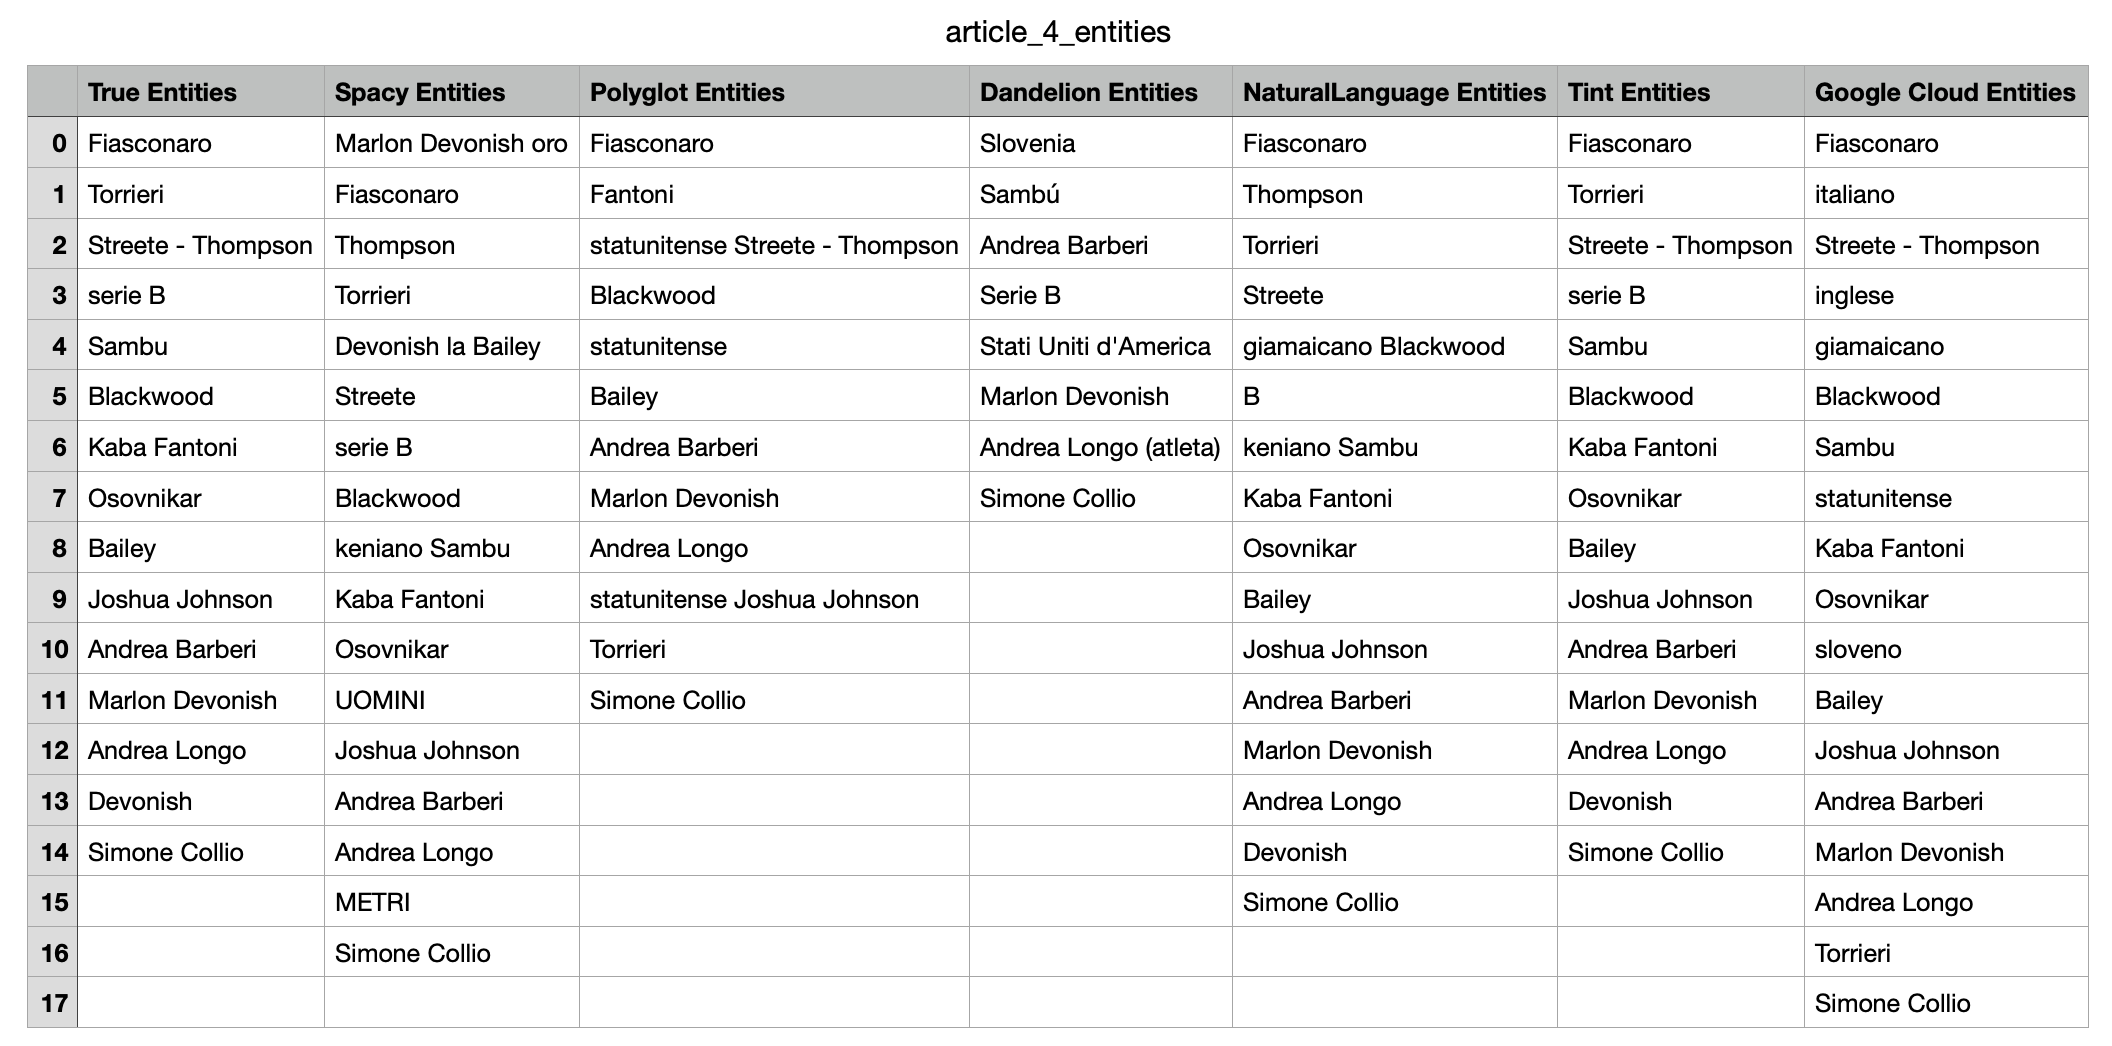
\includegraphics[width=0.9\textwidth]{img/entities_table}
\caption{Tabella di comparazione delle entità trovate nell'articolo di figura \ref{fig:article_4}.}
\label{fig:entities_table}
\end{figure}

\begin{figure}[H]
\centering
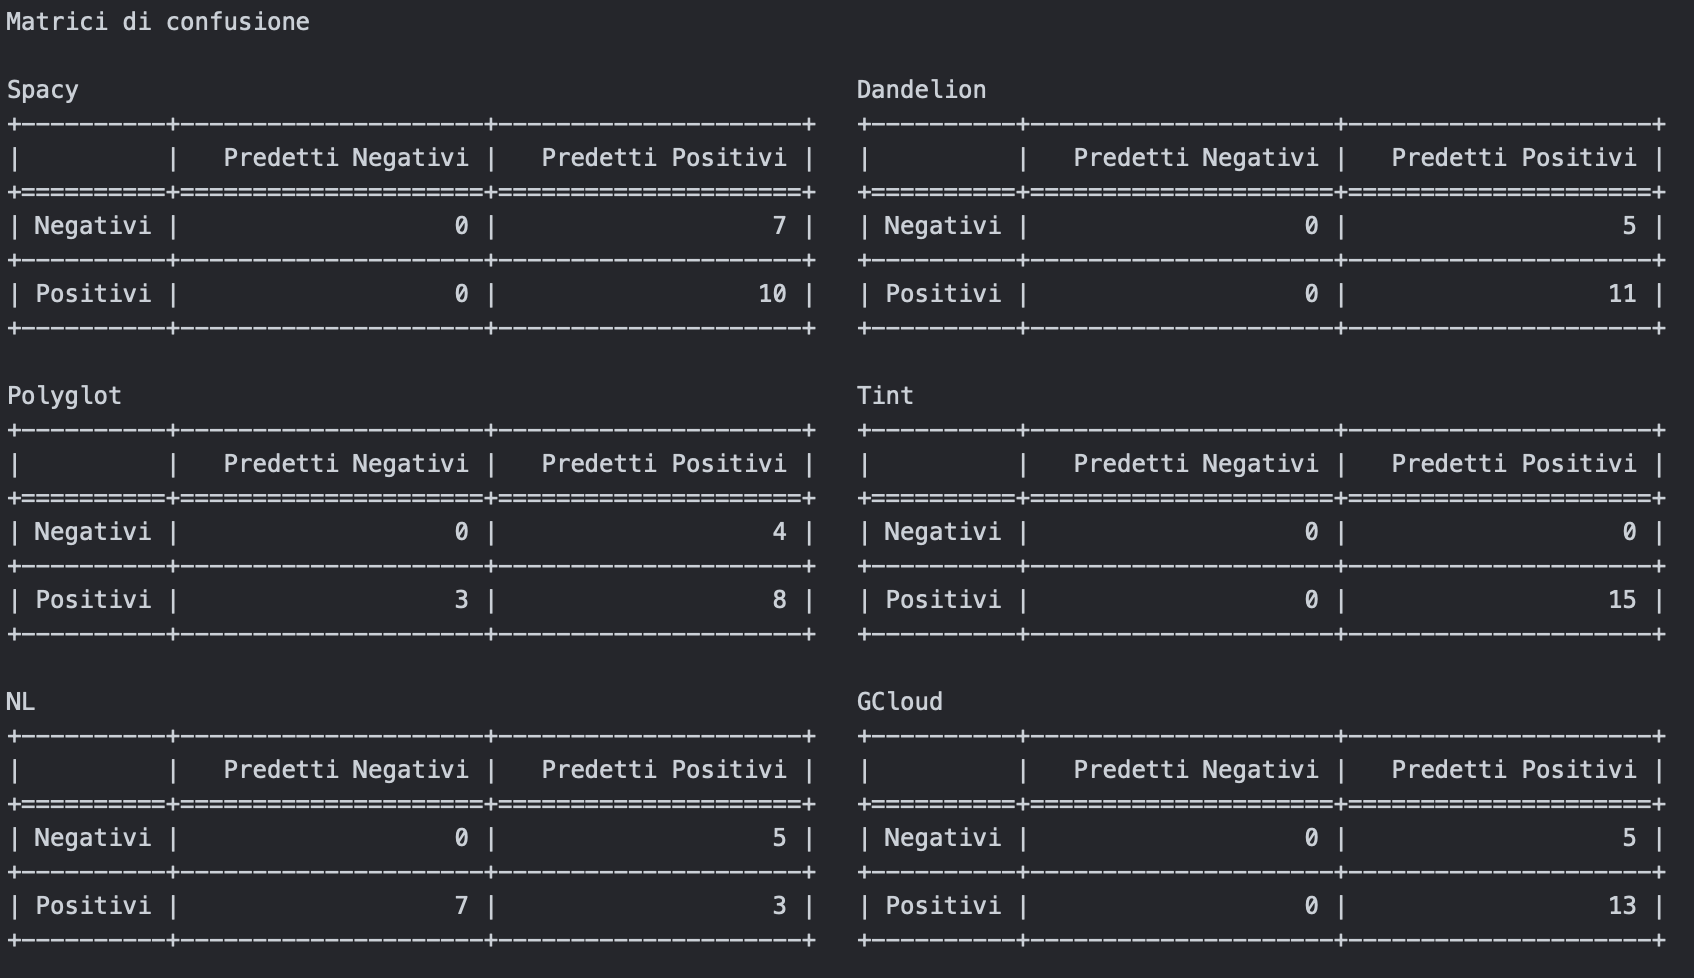
\includegraphics[width=0.9\textwidth]{img/matrici_confusione}
\caption{Matrici di confusione per ciascun tool relative all'articolo di figura \ref{fig:article_4}.}
\label{fig:confusion_matrixes}
\end{figure}

\begin{figure}[H]
\centering
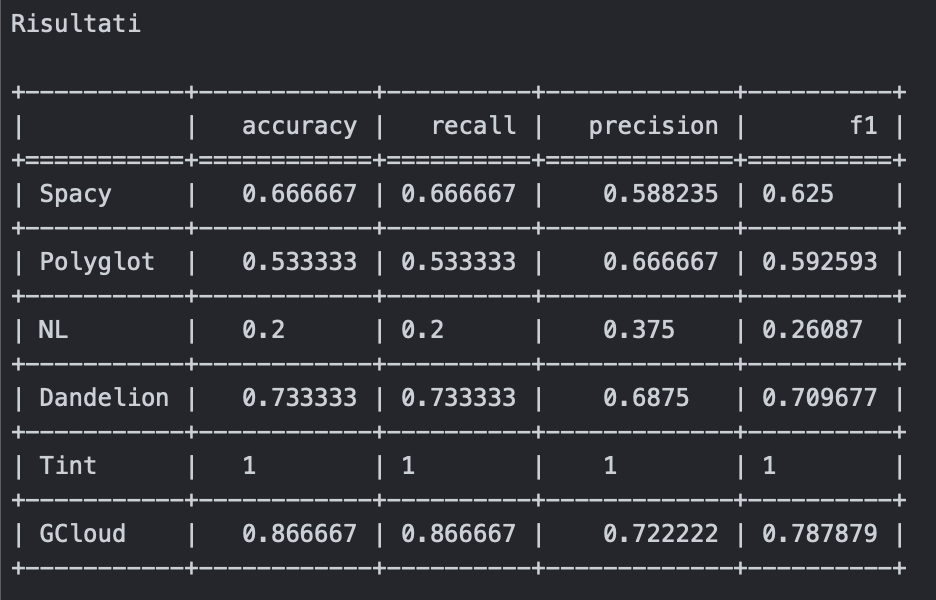
\includegraphics[width=0.8\textwidth]{img/results_ex}
\caption{Metriche calcolate per ciascun tool sull'articolo di figura \ref{fig:article_4}..}
\label{fig:results_ex}
\end{figure}

I risultati per questo esperimento, ottenuti come la media calcolata su tutti gli articoli, sono illustrati nel capitolo \ref{results-performance}.

\subsection{Tempi di computazione}
Il secondo esperimento realizzato ha lo scopo di valutare i tempi di computazione per ciascun tool. Sono stati quindi misurati i tempi di estrazione di entità di ciascun tool su 50 articoli diversi ed è stata poi fatta la media.

È importante sottolineare però che nel caso di \textit{Dandelion} (\ref{extractor:dandelion}), \textit{Google Cloud} (\ref{extractor:gcloud}) e \textit{Tint} (\ref{extractor:tint}) questi risultati sono poco rilevanti, in quanto si tratta di tool che operano tramite API \textit{REST} in cui il tempo di estrazione dipende soprattutto dai tempi di risposta del server.

Nel caso degli altri tool, è stato anche ignorato l'eventuale tempo necessario a caricare i modelli in memoria e, nel caso di \textit{Tint}, il tempo di attesa per l'avvio del server locale.

I risultati ottenuti per questo esperimento sono illustrati nel capitolo \ref{results-times}.

\subsection{Specifiche hardware}
Tutti gli esperimenti sono stati effettuati su un \textit{MacBook Pro (Retina, 13-inch, Mid 2014)} con processore 2,6 GHz Dual-Core Intel Core i5 e 8 GB di RAM (1600 MHz DDR3), con sistema operativo \textit{macOS Catalina} (versione 10.15.6).

Sulla macchina è installato \textit{Python} versione 3.7.6 e \textit{Java} versione 13.0.2.

L'IDE utilizzato è \textit{Pycharm (Professional Edition)} versione 2020.2.

% Risultati
\addtocontents{toc}{\protect\setcounter{tocdepth}{2}}
\clearpage
\section{Risultati ottenuti}
\label{sec:results}

\subsection{Valutazione della performance}
\label{results-performance}

Di seguito è riportata la tabella della media delle metriche (accuracy, recall, precision e f1 score) calcolate per ciascun tool su 50 articoli in lingua \textbf{inglese}:
% Tabella EN
\begin{table}[H]
\centering
{\renewcommand{\arraystretch}{1.35}%
\begin{tabular}{|l|r|r|r|r|}
\hline
{} &  \textbf{accuracy} & \textbf{recall} & \textbf{precision} & \textbf{f1 score} \\\hline
\textbf{Spacy    } &   0.66701 &   0.66701 &  0.637997 &  0.649229 \\\hline
\textbf{Polyglot } &  0.558444 &  0.558444 &  0.521301 &   0.53556 \\\hline
\textbf{NL       } &  0.705091 &  0.705091 &  0.682237 &   0.68868 \\\hline
\textbf{Dandelion} &  0.545663 &  0.545663 &  0.525791 &  0.528783 \\\hline
\textbf{NLTK     } &  \textbf{0.723784} &  \textbf{0.723784} &  0.575887 &  0.637886 \\\hline
\textbf{Stanford } &  0.655325 &  0.655325 &  \textbf{0.707102} &  \textbf{0.674614} \\\hline
\textbf{GCloud   } &  0.651893 &  0.651893 &   0.62159 &  0.632342 \\\hline
\textbf{Stanza   } &  0.684041 &  0.684041 &  0.645705 &  0.660724 \\
\hline
\end{tabular}}
\caption{\label{tab:en-results}Tabella delle performance dei tool per l'estrazione di entità in lingua inglese.}
\end{table}

Di seguito sono riportati gli stessi dati ma in forma di istogramma:

% Metriche EN
\begin{figure}[H]
\centering
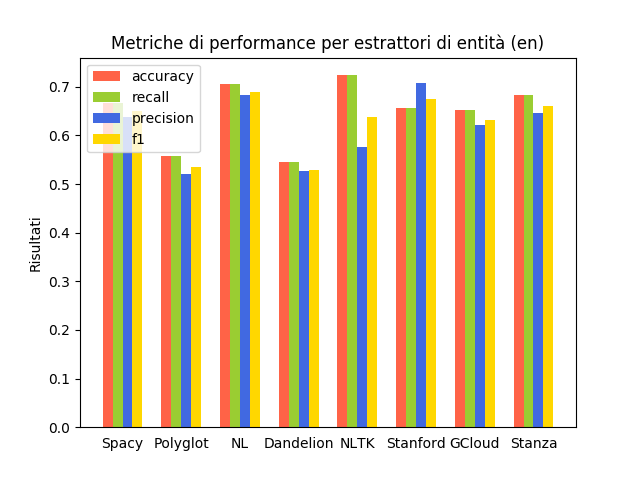
\includegraphics[width=0.8\textwidth]{img/results-en}
\vspace*{-5mm}
\caption{Istogramma relativo ai dati della tabella \ref{tab:en-results}.}
\label{fig:results-en}
\end{figure}

\clearpage
Di seguito invece è riportata la tabella della media delle metriche (accuracy, recall, precision e f1 score) calcolate per ciascun tool su 50 articoli in lingua \textbf{italiana}:

% Tabella IT
\begin{table}[H]
\centering
{\renewcommand{\arraystretch}{1.35}%
\begin{tabular}{|l|r|r|r|r|}
\hline
{} &  \textbf{accuracy} & \textbf{recall} & \textbf{precision} & \textbf{f1 score} \\\hline
\textbf{Spacy    } &  0.591253 &  0.591253 &  0.616677 &  0.595456 \\\hline
\textbf{Polyglot } &   0.45896 &   0.45896 &  0.473719 &   0.46029 \\\hline
\textbf{NL       } &  0.517147 &  0.517147 &  0.585914 &  0.538017 \\\hline
\textbf{Dandelion} &  0.287502 &  0.287502 &  0.496723 &   0.34487 \\\hline
\textbf{Tint     } &  \textbf{0.802747} &  \textbf{0.802747} &   \textbf{0.80021} &   \textbf{0.79569} \\\hline
\textbf{GCloud   } &  0.622233 &  0.622233 &  0.643944 &  0.625301 \\
\hline
\end{tabular}}
\caption{\label{tab:it-results}Tabella delle performance dei tool per l'estrazione di entità in lingua italiana.}
\end{table}

E in forma di istogramma:
% Metriche IT
\begin{figure}[H]
\centering
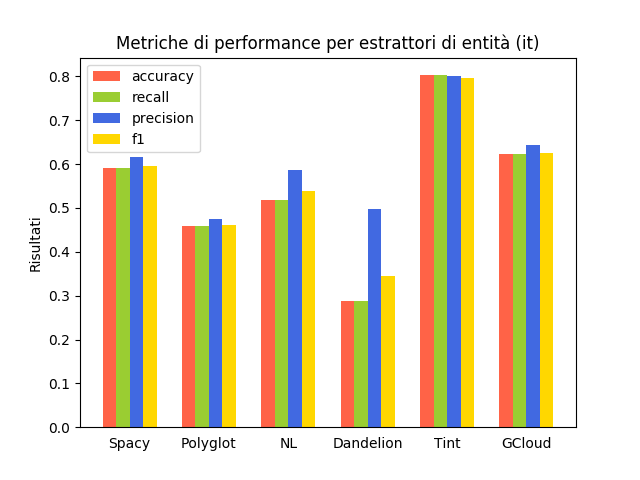
\includegraphics[width=0.8\textwidth]{img/results-it}
\vspace*{-5mm}
\caption{Istogramma relativo ai dati della tabella \ref{tab:it-results}.}
\label{fig:results-it}
\end{figure}

È importante però sottolineare che il risultato per \textit{Tint} non è imparziale, in quanto il classificatore incluso in \textit{Tint} è allenato sullo stesso dataset scelto per l'elaborato \cite{dataset-it}. Questo porta sicuramente a problemi di sovradattamento (\textit{overfitting}) e accuratezza più alta del normale.

Per quanto riguarda gli scarsi risultati di \textit{Dandelion}, invece, c'è da dire che i valori ottenuti dipendono fortemente dalla soglia di confidenza scelta, e che le entità restituite dal servizio, oltre a luoghi, persone e organizzazioni, includono anche concetti astratti (es. "arte", "musica", "sport") che non è possibile escludere.

\subsection{Tempi di computazione}
\label{results-times}
Di seguito sono mostrate le medie dei tempi di estrazione di entità per ciascun tool. L'estrazione va considerata calcolata su un breve articolo di dieci frasi, si a in inglese che in italiano.
%Tempi EN
\begin{figure}[H]
\centering
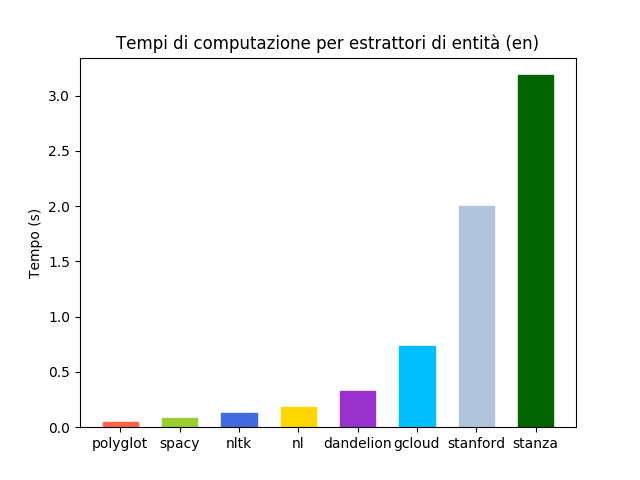
\includegraphics[width=0.8\textwidth]{img/time-en}
\vspace*{-5mm}
\caption{Tempi di estrazione di entità in lingua inglese.}
\label{fig:time-en}
\end{figure}

% Tempi IT
\begin{figure}[H]
\centering
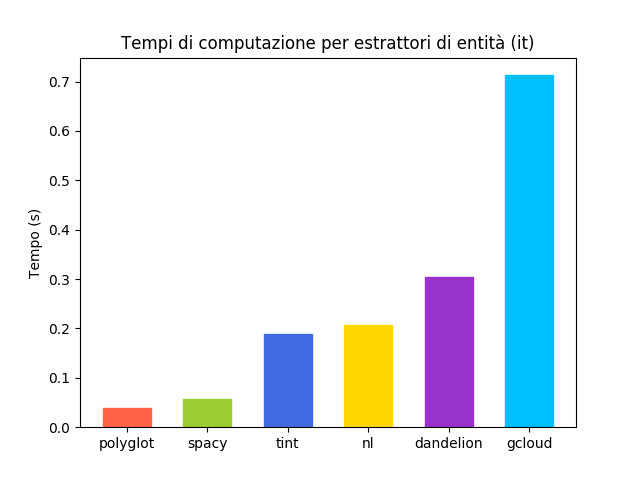
\includegraphics[width=0.8\textwidth]{img/time-it}
\vspace*{-5mm}
\caption{Tempi di estrazione di entità in lingua italiana.}
\label{fig:time-it}
\end{figure}

Come già detto in precedenza, i tempi sono esclusivamente quelli di estrazione di entità: sono stati esclusi tempi di caricamento dei modelli o di attesa di avvio del server locale.

\subsection{Conclusioni e sviluppi futuri}
In generale, stabilire quale sia il tool migliore in base alle metriche (\textit{accuracy, recall, precision, f1}) \textbf{dipende fortemente dallo scopo del progetto}: un estrattore con buona \textit{accuracy} e \textit{recall}, ma \textit{precision} bassa (come nel caso di \textit{NLTK} nel dataset inglese) è utile se lo scopo è quello di identificare tutte le possibili entità nel testo, a costo di trovarne anche altre "false". Viceversa, un estrattore con \textit{precision} alta (come \textit{Dandelion} nel dataset italiano) si adatta bene se si vuole trovare solo entità che hanno un'alta probabilità di verità, a costo di perdere alcune informazioni.
\newline

Ci sono in realtà dei problemi legati alla misura della qualità dell'output di un estrattore di entità. 
Uno di questi è legato alla presenza di \textbf{match parziali}, che non dovrebbero essere considerati nè come successi e nè come fallimenti completi. Ad esempio, se una frase cita il "Parco Nazionale dello Stelvio", è possibile che un estrattore in output restituisca soltanto l'entità "Stelvio" (comune di Bolzano): per le metriche definite prima, questo risultato viene considerato totalmente sbagliato nonostante abbia comunque a che fare con l'entità originale. 

Si potrebbe pensare semplicemente di contare la frazione di token identificata correttamente all'interno dell'entità (l'estrazione di "Stelvio" al posto di "Parco Nazionale dello Stelvio" in questo caso conterebbe come 1/4 = 0.25, invece di zero). 

Questo può però portare ad un'altra serie di problemi, uno tra tutti dato dal fatto che non è detto che parte di un'entità sia legato all'entità stessa (ad esempio, l'entità "Istituto Agrario di San Michele" in provincia di Trento non ha niente a che fare con "San Michele" arcangelo).
\newline

Per quanto riguarda i possibili sviluppi futuri, potrebbe essere interessante valutare i tool anche in base al \textit{tipo} di entità estratta (persona, organizzazione o luogo) e verificare che coincida con quello vero. Un altro sviluppo potrebbe essere quello di occuparsi, oltre al riconoscimento di entità, anche di \textbf{Named Entity Linking} (\textit{NEL}), ovvero quella parte di elaborazione del linguaggio naturale che si occupa di assegnare un'identità univoca (come ad esempio un \textit{URI}) e disambiguare le entità trovate.

%% Bibliography
\clearpage
\bibliography{bibliography.bib}
\bibliographystyle{ieeetr}

\end{document} 